% !TEX root = ../main.tex
\chapter{Another chapter}
\label{ch2}


\section[Section with long title]{A section with a
ridiculously long title for testing overflow}
\label{sec:ch2_long_title}


A figure, stored in \texttt{figs/} and referenced as
Figure~\ref{fig:loss-landscape}.

\begin{figure}[t]
  \centering
  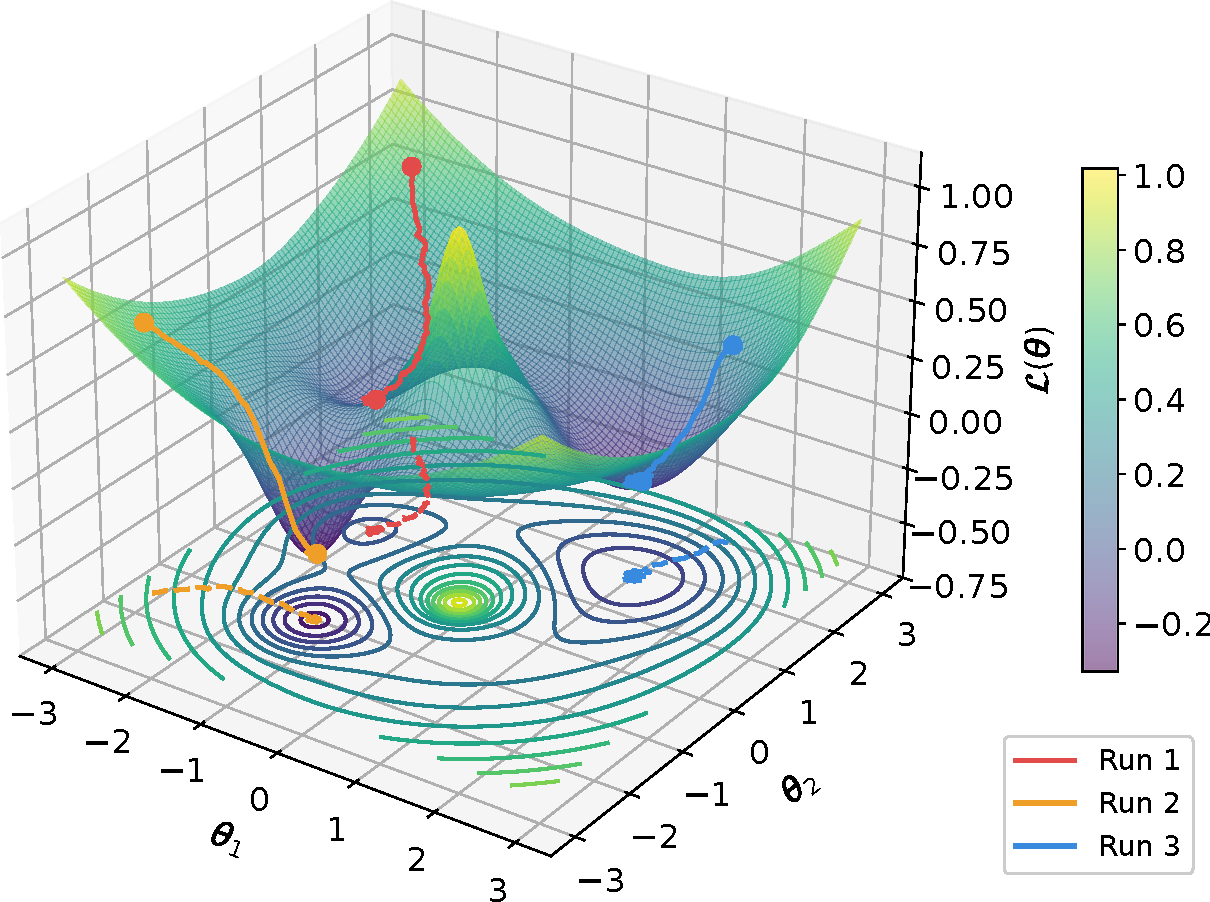
\includegraphics[width=0.8\linewidth]{figs/loss_landscape_sgd.pdf}
  \caption[Non-convex loss function 3D visualization]{3D visualization of
  a non-convex loss function $\mathcal{L}(\theta)$ with $\theta = \{\theta_1,
  \theta_2\}$, with three separate SGD optimization runs, starting from
  different $\theta$ initializations.
  }
  \label{fig:loss-landscape}
\end{figure}


An equation
\begin{equation}
f(a) = \frac{e^{a_i}}{\sum_{k}^{} e^{a_k}}
\end{equation}

Citations in different formats: \citep{lane2019natural} and
\citet{jones1972statistical}. A reference to
Section~\ref{ch1:sec:outline}.

\subsection{A sub-section}
\label{sub:sub}

\begin{table}[t]
\centering
  \begin{tabular}{lc}
 \hline
 \bf Word & \bf One-hot vector\\
 \hline
 andrew & [1, 0, 0, 0, 0] \\
 is & [0, 1, 0, 0, 0] \\

 a & [0, 0, 1, 0, 0] \\

 sweet & [0, 0, 0, 1, 0]\\

 guy & [0, 0, 0, 0, 1]\\
 \hline
\end{tabular}
\caption{A table.}
\label{tab:wordnvec}
\end{table}

A footnote.%
\footnote{With a URl \url{www.duckduckgo.com}.}

\todo{A todo note in the margin}

\todo[inline]{An in-line todo note}
